\chapter{SQL Injection (SQLi)}
\section{Popis}
SQL Injection podobně jako XSS využívá neochráněných vstupů, ovšem cílem je napadání databázové vrstvy (viz dříve). Pomocí neochráněných vstupů jsme schopni upravovat SQL dotazy, vkládat do nich podmínky, popřípadě vnořené dotazy.

\section{Příklad SQL Injection}
Mějme tabulku (například v databázovém systému \textit{MySQL}) se seznamem písniček. Ukázku tabulky můžeme vidět v tabulce:
\begin{table}[!h]
\centering
\begin{tabular}{|c|c|l|l|}
\hline
\bf id & \bf category$\_$id & \bf autor & \bf name \\
\hline
\hline
\bf 1. & \bf 2 & Celldweller & One good reason \\
\hline
\bf 2. & \bf 3 & Asonance & Království Keltů \\
\hline
\bf 3. & \bf 2 & Celldweller & EON \\
\hline
\bf 4. & \bf 4 & Hectix & Return \\
\hline
\bf 5. & \bf 3 & Blue Stahli & Takedown\\
\hline
\end{tabular}
\label{tab:hac}
\caption{Tabulka hudebního katalogu}
\end{table}
\newline
Ve webové aplikaci přejdeme na URL:
\begin{lstlisting}[label=web_app_url_1,language=HTML, caption=URL webové aplikace]
http://localhost/songs.php?categoryId=2
\end{lstlisting}

Script \textit{songs.php} načte parametr \textit{categoryId} a podle něj vytvoří dotaz, který vybere písničky z dané kategorie:

\begin{lstlisting}[label=web_app_url_2,language=SQL, caption=Vytvořený SQL dotaz]
SELECT * FROM songs WHERE category_id = 2
\end{lstlisting}

Dotaz bude vykonán a na webové stránce se zobrazí pouze písničky z~kategorie číslo 2. Pokud bychom ale URL ručně přepsali a nahradili bychom kritickou část, například:
\begin{lstlisting}[label=web_app_url_3,language=HTML, caption=Ručně upravené URL]
http://localhost/songs.php?categoryId = 2 OR 1 = 1
\end{lstlisting}

a script by nebyl ochráněn proti těmto \uv{nevhodným} vstupům, zachoval by se stejně a vygeneroval by následující dotaz:
\begin{lstlisting}[label=web_app_url_4,language=SQL, caption=Vygenerovaný SQL dotaz z upraveného URL]
SELECT * FROM songs WHERE category_id = 2 OR 1 = 1
\end{lstlisting}

Tento dotaz je ovšem úplně jiný, vrací totiž všechny skladby.

\section{Rozdíl mezi SQL Injection a Blind SQL Injection}
Podstata útoku je v obou případech stejná, ovšem u \textit{Blind SQL Injection} nevidíme výsledek, což znamená delší hledání problému. Oproti tomu v předchozím případě jsme výsledek viděli ihned (zobrazily se všechny skladby a ne pouze daná kategorie), což znamenalo odhalení tohoto problému. 

\section{Předcházení a obrana}
\begin{itemize}
\item Kontrola příchozích dat na aplikační vrstvě - pokud vím, že mi v parametru \textit{category\_id} má přijít číslo, tak budu validovat číslo.
\item Využití funkcí pro \uv{přepsání} speciálních znaků do entit (v php např.: \textit{mysql\_real\_escape\_string} \ldots). Tyto funkce nahradí znaky, které by mohly SQL dotaz nějakým způsobem \textit{upravit} nebo \textit{poškodit} na text.
\item Využití databázové vrstvy, která má jako jeden z cílů právě předcházení těmto rizikům (příkladem může být \textit{Dibi - Database Abstraction Library pro PHP}\footnote{Je zdarma k dispozici na http://dibiphp.com}).
\item Správně nastavená oprávnění - pro připojení webových aplikací využívat speciálního uživatele s omezenými právy (pokud je z nějakého důvodu nepotřebujeme). Ideálně aplikace a k ní konkrétní uživatel s~jednou databází, který nikam jinam nemůže (zabránění, aby se z DB jedné aplikace dostal i do dalších), dále zákaz nepotřebných příkazů pro tyto uživatele (například exec, drop, alter). Pak i kdyby útočník objevil SQL Injection chybu, tak nám například nemůže vymazat všechny tabulky.
\end{itemize}

\chapter{Důsledky}
Důsledky napadení nedostatečně zabezpečené aplikace mohou být fatální, ať je to získání administrátorského přístupu do webové aplikace, odcizení dat nebo až získání úplné kontroly nad cílovým serverem.

\section{Ukázky možného napadení}
\subsection{SQLi v redakčním systému}
Tato chyba byla nahlášena na \textit{http://exploit-db.org/} a její kód zveřejněn. Byly zasaženy desítky webů používajících redakční systém WordPress. Z obrázku je vidět, že parametr \textit{id} není bezpečný, tudíž je možné dotaz upravit a získat například uživatelská jména či  hesla.
\begin{figure}[h!]
\centering{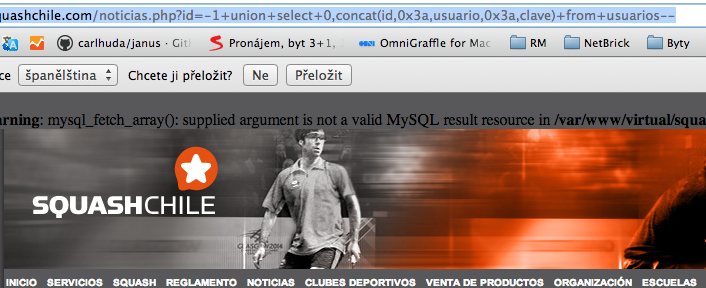
\includegraphics[width=390px]{./examples/squash-sqli.png}}
\caption{SQL injection v redakčním systému}
\label{obr.squash}
\end{figure}

\subsection{Chybný přihlašovací formulář}
Ukázka chybně zabezpečného vstup přihlašovacího formuláře na nejmenovaném portálu české firmy, kde je možné se pomocí zakomentování zbytku SQL dotazu (ověření hesla) přihlásit jako administrátor.
\begin{figure}[h!]
\centering{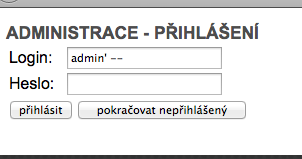
\includegraphics[width=282px]{./examples/login_test.png}}
\caption{Zápis SQLi}
\label{obr.login1}
\end{figure}

\begin{figure}[h!]
\centering{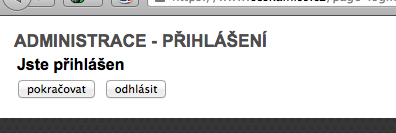
\includegraphics[width=346px]{./examples/login_suc.png}}
\caption{Úspěšné přihlášení}
\label{obr.login2}
\end{figure}


\subsection{Sony Pictures - 2011}
Proti společnosti Sony byly v roce 2011 několikrát použity DDoS útoky a nakonec vše vyústilo v odcizení dat skupinou LulzSec\footnote{Lulz Security - skupina počítačových hackerů, jejich webové stránky byly zablokovány, ale twitter zůstal \textit{https://twitter.com/LulzSec}} pomocí SQL injection. I taková velká společnost jako Sony, měla údaje v databázích v nešifrované podobě. Hackerům se podařilo odcizit 1 milion uživatelských dat (jména, hesla, adresy a datum narození), dále hesla administrátorů a mnoho dalšího - více v \textit{http://www.thewhir.com/web-hosting-news/hackers-attack-sony-pictures-with-single-sql-injection}. Většina členů této skupiny byla nedávno zatčena a pochytána, díky chybě hlavního člena s přezdívkou \uv{Sabu} a jeho následné spolupráci s FBI zdroj \textit{The Guardian}\cite{guardian}.

\begin{center}
\textit{You call it war, we laugh at your battleships.}\\
(Heslo skupiny LulzSec)
\end{center}
